\chapter{Verwendete Technologien}
\label{chap:technologien}

\section{WebGL}
\label{sec:webgl}
3D-Szenen im Webbrowser darzustellen wurde 1997 zuerst von den Ingenieuren von SGI (Silicon Graphics Incorporated) versucht \autocite[110]{Zielgerichtet}. Die damaligen Heimcomputer waren dafür aber hardwaremäßig viel zu schwach ausgestattet, sodass die Anwendungen hauptsächlich auf teuren dedizierten Workstations liefen. Dennoch wurde der Ansatz weiterverfolgt und ein Konsortium entwickelte den ISO-Standard VRML97. Dieser war jedoch für Entwickler schwer zu handhaben und ließ sich nicht gut in die Webseite integrieren. Daher fand er nur eine geringe Verbreitung. Das Konsortium entwickelte die Idee jedoch weiter und veröffentlichte X3D\footnote{\url{http://www.web3d.org/realtime-3d/x3d/what-x3d/} (besucht am \today)}, ein XML-basiertes Beschreibungsformat für 3D-Szenen. Auch dieses blieb aber eine Nischenlösung.

Einen wirklichen Durchbruch für interaktive 3D-Inhalte im Webbroswer könnte WebGL bringen, welches von den meisten modernen Browsern bereits vollumfänglich unterstützt wird (auch wenn die Unterstützung häufig noch als experimentell deklariert ist). Es lässt sich in den folgenden Browsern verwenden:
\begin{itemize}
    \item Google Chrome ab Version 9
    \item Mozilla Firefox ab Version 4
    \item Safari ab Version 5.1 (muss manuell aktiviert werden)
    \item Opera ab Version 11
\end{itemize}
Microsoft hat derzeit noch keine Pläne angekündigt WebGL in den Internet Explorer zu integrieren.

WebGL ist ein Application Programming Interface (API) basierend auf OpenGL ES 2.0, dem OpenGL-Standard für mobile Endgeräte \autocite{OpenGlES}, und wird von der Khronos Group aktiv entwickelt. Die Khronos Group ist ein Non Profit-Konsortium das sich mit der Entwicklung von Standards für Computergrafik, nebenläufige Programmierung, dynamische Medien und andere Themenfelder befasst. Die Spezifikation für die Version 1.0 ist im Februar 2011 erschienen \autocite{WebGLSpec}. Es basiert zwar auf OpenGL ES 2.0, allerdings gibt es einige kleine Unterschiede deren man sich gewahr sein muss wenn man aus dem OpenGL ES-Umfeld kommt (siehe \autocite{WebGLDiff}). Für die Programmierung wird JavaScript direkt verwendet oder eine Sprache die nach JavaScript kompiliert (beispielsweise CoffeeScript\footnote{\url{http://coffeescript.org} (besucht am 16. August 2012)} oder Dart\footnote{\url{http://www.dartlang.org} (besucht am 16. August 2012)}). Die Grundlage für das Zeichnen in WebGL ist das HTML5-Element \textit{canvas}. Aus diesem Grund wird WebGL auch häufig zum HTML5-Standard dazugezählt, ist aber bis auf die Abhängigkeit vom Canvas-Elements völlig eigenständig.

Eine WebGL-Anwendung besteht, wie die meisten Webanwendungen, aus HTML-Seiten, JavaScript- sowie CSS-Dateien und wird in einem Webbrowser ausgeführt. Im Gegensatz zu den herkömmlichen Methoden 3D im Browser darzustellen (X3D, Flash, etc.) hat WebGL den großen Vorteil, dass kein spezielles Plugin benötigt wird. Die Unterstützung ist nativ in die Browser eingebaut. Informationen über die darzustellenden Inhalte sowie die Art und Weise wie diese dargestellt werden, werden über JavaScript direkt an die WebGL-API weitergegeben. Zu diesen Informationen gehört neben den darzustellenden Inhalten auch WebGL-spezifischer Inhalt, wie der Code für die verwendeten Shader.
\begin{figure}
\centering
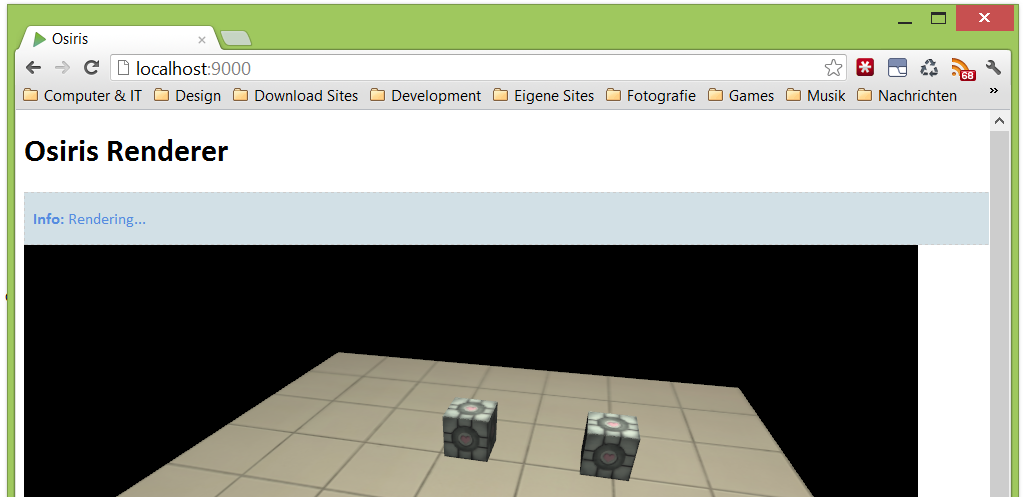
\includegraphics[width=\textwidth]{bilder/canvas.png}
\caption{3D-Szene gerendert im Canvas mit WebGL}
\label{fig:webglcanvas}
\end{figure}
\begin{figure}
\centering
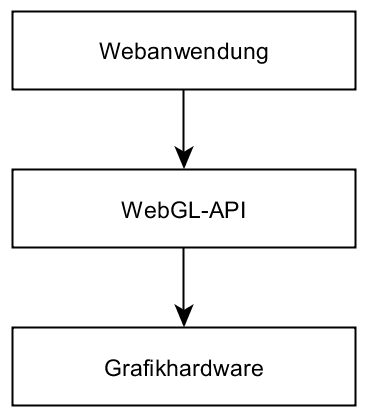
\includegraphics[height=50mm]{bilder/webglflow.png}
\caption{Befehlsfluss in einer WebGL-Anwendung}
\label{fig:webglflow}
\end{figure}
In den folgenden Abschnitten werde ich die wichtigsten Elemente vorstellen, die für das Verstehen einer WebGL-Anwendung unerlässlich sind.

\subsection{Der Kontext}
Das HTML5-Canvaselement stellt verschiedene Kontexte bereit, über die man den dargestellten Inhalt manipulieren kann. Der WebGL-Kontext hat, je nach Browserhersteller, derzeit noch verschiedene Namen. Allerdings soll dies zukünftig auf "`webgl"' standardisiert werden. Mit Hilfe der Bibliothek \textit{WebGLUtils}\footnote{\url{https://cvs.khronos.org/svn/repos/registry/trunk/public/webgl/sdk/demos/common/webgl-utils.js} (besucht am 16. August 2012)} von Google reicht allerdings ein einzelner Funktionsaufruf.

Der WebGL-Kontext enthält alle Funktionsaufrufe an die WebGL-API und ist somit die direkte Verbindung zur Grafikhardware des Computers. Daher ist er an sehr vielen Stellen innerhalb der Anwendung von enormer Bedeutung.

Durch verschiedene Ereignisse kann der Kontext verloren gehen. Die Grafikhardware ist eine geteilte Ressource und kann plötzlich von anderen Prozessen in Anspruch genommen werden oder eine WebGL-Anwendung erzeugt einen Timeout, wodurch der Grafikkartentreiber die Hardware zurücksetzt. Es gibt viele Gründe warum der Kontext verloren gehen kann. Wichtig ist nur zu verstehen, dass es jederzeit passieren kann, wodurch die Anwendung dann nicht mehr funktionieren wird. Daher muss unbedingt darauf geachtet werden, dass eine WebGL-Anwendung auf den Kontextverlust angemessen reagiert. Das Canvas-Element bietet hierfür zum einen die Möglichkeit zwei Eventlistener zu registrieren. Ein Eventlistener reagiert auf das \textit{webglcontextlost}-Event was, wie der Name schon sagt, ausgelöst wird sobald der Kontext verloren geht. Der zweite Eventlistener reagiert auf \textit{webglcontextrestored} und zeigt an, dass der Kontext wiederhergestellt wurde. Zum anderen ist es möglich über die Funktion \texttt{isContextLost} jederzeit den Zustand des Kontexts abzufragen.

\subsection{Shader}
Wie OpenGL ES 2.0 ist auch WebGL rein shaderbasiert. Shader sind kleine Programme die die eingehenden Informationen (3d-Modelldaten, Texturen, Beleuchtung etc.) verarbeiten und, je nach programmiertem Verhalten, bestimmen was letztendlich auf dem Canvas zu sehen sein wird. Sie werden direkt auf der Grafikhardware ausgeführt und erlauben somit eine sehr flexible und performante Darstellung der Szene.

In WebGL ist man auf zwei Shadertypen beschränkt: den Vertex- und den Fragmentshader. Diese werden in der OpenGL ES Shading Language (GLSL ES) geschrieben und müssen vor Gebrauch kompiliert und zu einem Shaderprogramm verbunden werden. Auch hierfür ist kein externer Compiler nötig. Dieser wird vom Grafikkartentreiber bereitgestellt und der Vorgang wird direkt vom Browser über JavaScript-Funktionsaufrufe der WebGL-API angestoßen (siehe Listing \ref{lst:createshaderfromsource}).
\lstset{language=JavaScript}
\begin{lstlisting}[caption={Erstellen eines Shaders (selbstgeschriebene Funktion)}, label={lst:createshaderfromsource}]
function createShaderFromSource(type, source) {
  var glShader = gl.createShader(type);
  gl.shaderSource(glShader, source);
  gl.compileShader(glShader);

  return glShader;
}
\end{lstlisting}
Der Shadercode muss als String an die Funktion \texttt{shaderSource} übergeben werden. Dies ist sehr flexibel, da man den Code so auf viele Arten in die Anwendung einbringen kann. So kann er beispielsweise in die HTML-Seite eingebunden oder direkt im JavaScript-Code festgelegt werden.

\subsection{Shaderaufbau}
Der Vertex- und Fragmentshader haben einen ähnlichen Aufbau. Zu Beginn müssen alle eingehenden und ausgehenden (nur Vertexshader) benutzerdefinierten Daten mit ihren Typen deklariert werden. Von der API können jedem der beiden Shader benutzerdefinierte \textit{Uniforms} mitgegeben werden. Uniforms sind Daten, die für alle Vertices\footnote{Ein Vertex ist ein Eckpunkt eines 3D-Modells.} pro Zeichnungsaufruf konstant bleiben, wie die Positionen und Farben von Lichtquellen oder Transformationsmatrizen.

Die GLSL ES ist eine an C angelehnte Sprache und bietet einen ausreichenden Satz von Features. Eigene Variablen können verwendet, in Structs zusammengefasst und Shaderlogik in Funktionen untergebracht werden. Zudem gibt es eine den meisten Programmierern wohlvertraute \texttt{main}-Funktion, innerhalb derer das Hauptprogramm abläuft. Die Hauptaufgabe eines Shaders ist es, "`seine"' spezielle globale Variable zu befüllen.

\subsubsection{Vertexshader}
Der Vertexshader hat die alleinige Aufgabe die 3D-Modelldaten (genauer: die Vertices) innerhalb der Szene zu manipulieren, d.h. in seinem Quelltext muss die globale Variable \texttt{gl\_Position} befüllt werden. Er wird immer zuerst ausgeführt und kann Berechnungsergebnisse (bsp. Normalentransformationen) an den Fragmentshader weitergeben. Dies geschieht über sogenannte \textit{Varyings}. Varyings sind von außen nicht zugreifbar. Zusätzlich zu den Uniforms können ihm pro Zeichenaufruf für jedes Vertex veränderliche Daten über \textit{Attributes} mitgeteilt werden. Dies sind beispielsweise die Position, die Normale, die Farbe etc.
\begin{figure}
\centering
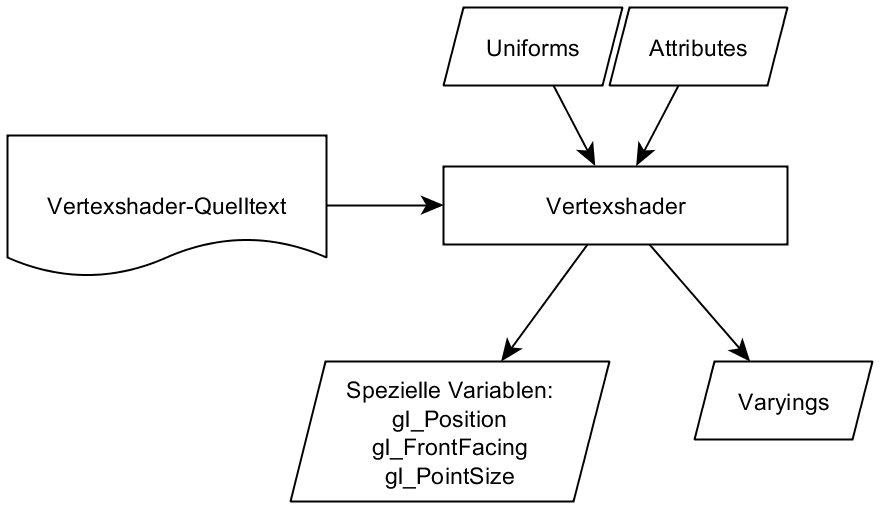
\includegraphics[height=60mm]{bilder/vertexshader.png}
\caption{Datenfluss in den und aus dem Vertexshader, nach \autocite{WebGlPogramming}}
\label{fig:vertexshader}
\end{figure}

\subsubsection{Fragmentshader}
Der Fragmentshader legt die Farbe eines Fragments\footnote{Ein Fragment entspricht einem Pixel auf dem Bildschirm, allerdings können in den nachfolgenden Fragmentoperationen der Rendering Pipeline einige Fragmente auch wieder verworfen werden. Daher die Unterscheidung zwischen Fragment und Pixel.} fest, d.h. in seinem Quelltext muss die globale Variable \texttt{gl\_FragColor} befüllt werden.

Neben den Uniforms und Varyings können dem Fragmentshader \textit{Sampler} übermittelt werden. Dies sind spezielle Uniforms, die für die Texturierung verwendet werden.

Am Anfang des Fragmentshader-Codes muss zwingend die Mindestpräzision für alle Fließkommaoperationen angegeben werden. In der Regel nutzt man hierfür die in Listing \ref{lst:fragmentshaderprecision} dargestellte Zeile.
\lstset{language=C}
\begin{lstlisting}[caption={Festlegen der Mindestpräzision für alle Fließkommaoperationen}, label={lst:fragmentshaderprecision}]
precision mediump float;
\end{lstlisting}
Dies ist vor allem für Anwendungen wichtig, bei denen die visuelle Qualität stark von der Genauigkeit der (unter Umständen sehr komplexen) Berechnungen abhängt. Allerdings kann die Wahl (\texttt{lowp}, \texttt{mediump} oder \texttt{highp}) auch Auswirkungen auf die Leistung haben oder wird von manchen Geräten (insbesondere im Mobilbereich) nicht unterstützt \autocite{WebGlPrecision}. Daher ist es ratsam immer entweder \texttt{lowp} oder \texttt{mediump} zu verwenden, je nach Anwendungsfall.
\begin{figure}
\centering
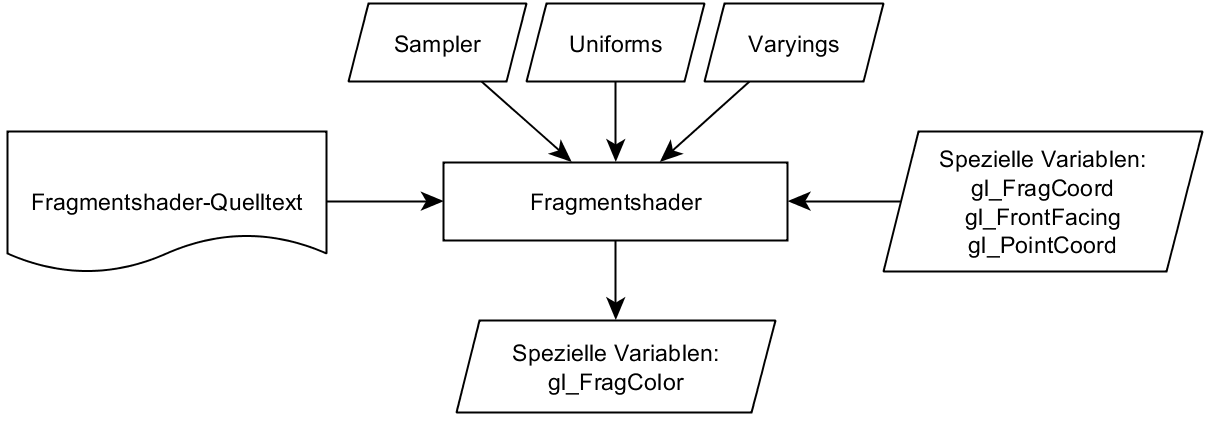
\includegraphics[width=\textwidth]{bilder/fragmentshader.png}
\caption{Datenfluss in den und aus dem Fragmentshader, nach \autocite{WebGlPogramming}}
\label{fig:fragmentshader}
\end{figure}

\subsection{Drawing Buffer}
Grafikkarten verfügen über einen Framebuffer in dem die Bilder (Frames), die später auf dem Monitor zu sehen sein werden, zusammengebaut werden. WebGL hat eine eigene Art von Framebuffer, den \textit{Drawing Buffer}. Wenn ein Renderzyklus erfolgreich abgeschlossen wurde und alle Daten die WebGL-Pipeline durchlaufen haben, wird aus ihnen im Drawing Buffer das fertige Bild erstellt. Dieses wird jedoch nicht direkt auf dem Monitor dargestellt, sondern mit dem Rest der HTML-Seite verbunden und dann an den Framebuffer der Grafikkarte gesendet. Dieser sendet es letztendlich an den Monitor \autocite[5--7]{WebGlPogramming}.

\section{WebSockets}
\label{sec:websockets}
Browser kommunizieren mit Servern über das Hypertext Transfer Protocol (HTTP). HTTP ist völlig statuslos und funktioniert nach dem Muster Request $\rightarrow$ Response. Alle Kommunikation geht hierbei vom Client aus, der eine Anfrage (Request) an den Server schickt. Dieser verarbeitet die Anfrage und sendet dem Client eine Antwort (Response). Hiernach schließt er die Verbindung und der Vorgang ist abgeschlossen. Dieses Verfahren ist für Echtzeit-Anwendungen jedoch aus folgenden Gründen problematisch:
\begin{itemize}
    \item HTTP erzeugt unnötigen Overhead \autocite[673]{WebsocketsFurukawa}. Da die Kommunikation statuslos ist werden bei jeder Anfrage viele Informationen mitgeschickt die für die eigentlich Aufgabe nicht benötigt werden, wie Header- und Statusinformationen. Dadurch ist der Server mit dem unnötigem Abarbeiten der immer gleichen und zu großen Informationspakete beschäftigt und kann so nicht seine volle Kapazität den anstehenden Berechnungen für den Client widmen. Zudem wird für jeden neuen Request eine komplett eigenständige HTTP-Verbindung in Gang gesetzt.
    \item Die Kommunikation ist unidirektional \autocite{WebsocketsRichter}. Da alle Kommunikation vom Client initiiert wird, hat der Server keine Möglichkeit den Client zu benachrichtigen sobald sich serverseitig Daten geändert haben. Erst bei der nächsten Anfrage würden die geänderten Daten geschickt werden. In einem Echtzeitsystem müsste der Client also den Server permanent anfragen (Pollen), was jedoch sowohl den Client als auch den Server unnötig belastet.
\end{itemize}
\begin{figure}
\centering
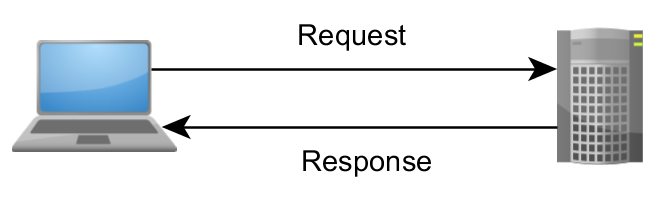
\includegraphics[width=80mm]{bilder/http.png}
\caption{Request/Response-Prinzip des HTTP-Protokolls}
\label{fig:http}
\end{figure}
Um das Problem der unidirektionalen Kommunikation teilweise zu lösen wurde das \textit{Comet}-Anwendungsmodell entworfen. Normalerweise sendet der Server bei unveränderten Daten eine leere Antwort und schließt dann die Verbindung. Ein Comet-Server lässt die Verbindung bei unveränderten Informationen zum Client jedoch so lange offen, bis neue Informationen da sind und sendet erst dann eine Antwort. Allerdings kann der Client keine neuen Informationen senden solange der vorige Request noch nicht beantwortet wurde und es wird immer noch für jeden Request eine eigene Verbindung aufgebaut \autocite[673]{WebsocketsFurukawa}.

In vielen Programmiersprachen wie Java, C/C++ oder C\# stehen dem Programmierer Konstruktionen für den Aufbau einer direkten TCP-Verbindung zum Server bereit. In JavaScript fehlte dies aufgrund der Beschränkung des Browsers auf HTTP bisher. Mit dem WebSocket API-Standard, der sich noch in der Entwicklung befindet (siehe \autocite{WebSocketApiSpec}), wird dieser Missstand jedoch zumindest teilweise behoben. Teilweise, da WebSockets immer auf der Anwendungsebene (Ebene 7) des ISO-OSI-Modells arbeiten \autocite{WebsocketsRichter} und so keine "`echten"' low-level Binärsockets darstellen. Der aktuelle Stand der Protokollspezifikation \autocite{WebSocketRFC} wird von folgenden Browsern unterstützt:
\begin{itemize}
    \item Google Chrome ab Version 16
    \item Mozilla Firefox ab Version 11
    \item Safari ab Version 6
    \item Internet Explorer ab Version 10
    \item Opera ab Version 12.50 (Entwicklerversion)
\end{itemize}
Aus der obigen Liste ist ersichtlich, dass für WebSockets ein noch aktuellerer Browser benötigt wird als für WebGL.

\subsection{Verbindungsaufbau}
Eine WebSocket-Verbindung startet immer als regulärer HTTP-Request. Dieser muss jedoch an eine Adresse gehen, die mit \textit{"`ws:\textbackslash\textbackslash"'} beginnt, statt mit \textit{"`http:\textbackslash\textbackslash"'}. Weiterhin muss der angesprochene Server das WebSocket-Protokoll auch unterstützen. Hiervon gibt es mittlerweile einige für unterschiedliche Programmiersprachen, wie die aktuellen Versionen der Jetty\footnote{\url{http://www.eclipse.org/jetty} (besucht am 17. August 2012)} und Glassfish\footnote{\url{http://www.oracle.com/technetwork/java/javaee/overview/index.html} (besucht am 17. August 2012)}-Server für Java oder PyWebsocket\footnote{\url{http://code.google.com/p/pywebsocket} (besucht am 17. August 2012)} für Python.\\
Ein WebSocket in der Clientanwendung zu initialisieren ist sehr leicht, wie Listing \ref{lst:websocketinit} zeigt.
\lstset{language=JavaScript}
\begin{lstlisting}[caption={Initialisieren einer WebSocket-Verbindung im Browser}, label={lst:websocketinit}]
var socket = new WebSocket("ws://HOST:PORT");

socket.onmessage = function(event) {
  // handle incoming messages
};

socket.onerror = function(error) {
  // handle errors with the connection
};

socket.onopen = function() {
  // the connection to the server has been establishes successfully
};

socket.onclose = function() {
  // the connection has been closed
};
\end{lstlisting}
Wie man sieht ist ein WebSocket über Callbacks eventgesteuert.

Das Socket sendet nun einen \textit{Upgrade}-Request inklusive einiger Zusatzinformationen (siehe \autocite{WebsocketsRichter}) als HTTP-Request an den WebSocket-Server. Wenn dieser die Verbindung annimmt, sendet er eine HTTP-Response und die Verbindung wird auf eine Full-Duplex\footnote{Gleichzeitiger Datenaustausch in beide Richtungen möglich} WebSocket-Verbindung aktualisert. Hierdurch wird das \textit{open}-Event ausgelöst und es können nun in Echtzeit Daten vom Client an den Server, sowie vice versa gesendet werden.
\begin{figure}
\centering
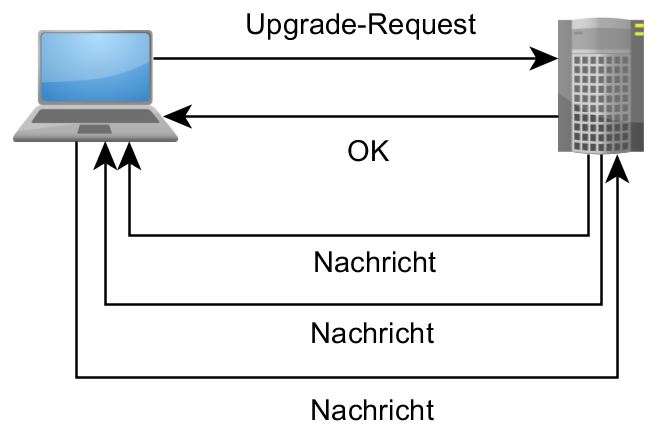
\includegraphics[width=80mm]{bilder/websocket.png}
\caption{Kommunikationsprinzip des WebSocket-Protokolls}
\label{fig:websocket}
\end{figure}

\subsection{Senden und Empfangen}
Sobald das \textit{open}-Event empfangen und somit das für \texttt{onopen} registrierte Callback ausgeführt wurde, lassen sich über die Methode \texttt{send} Daten als Strings an den Server schicken. Der Server kann von sich aus jederzeit Daten senden, wodurch das \textit{message}-Event ausgelöst und damit das für \texttt{onmessage} registrierte Callback aufgerufen wird. Über den \texttt{event}-Parameter des Callbacks lässt sich die Property \texttt{event.data} auslesen, welche die Nachricht des Servers als String beinhaltet.

\section{Realtime Interactive System}
\label{sec:ris}
Ein Realtime Interactive System (kurz RIS) ist ein System mit dem man in Echtzeit interagieren kann, welches also Eingaben sofort verarbeitet und die Ergebnisse zurückliefert. Das prominenteste Beispiel (und ein Spezialfall) hierfür sind wohl Computerspiele. In einem RIS werden in aller Regel verschiedenartige Komponenten miteinander verbunden wie eine 3D-Engine, eine Physik-Engine, eine AI-Engine\footnote{Artifical Intelligence (Künstliche Intelligenz)} und möglicherweise noch einige mehr. Drei für ein RIS typische Architekturmerkmale sind ein Szenengraph, ein Eventsystem und ein Entitymodell \autocite[299]{GuruMeditation}. Das RIS kümmert sich dann unter anderem darum, dass die Komponenten miteinander kommunizieren können. Dies ist wichtig, da beispielsweise die 3D-Engine die Transformationsdaten für die dargestellten Objekte von der Physik erhalten und der Handler für Tastatur- und Mauseingaben der Physik mitteilen können muss, welches Objekt gerade vom Benutzer manipuliert wird. Bei der Entwicklung arbeiten häufig verschieden spezialisierte Teams an den einzelnen Komponenten. So wird die 3D-Engine von Grafikprogrammierern, die AI-Engine von AI-Programmierern entwickelt. Schon am Anfang stellt sich für alle Teams das Problem die Programmierschnittstelle der eigenen Komponente für andere Komponenten zu definieren. Da sich die Ein- und Ausgabedaten in der Regel unterscheiden ist es oft mit erheblichem Aufwand verbunden im Nachhinein eine Komponente gegen eine andere auszutauschen. Im Folgenden werden einige relevante Dinge zu SIRIS erläutert, dem für diese Arbeit gewählten RIS.

\subsection{SIRIS}
SIRIS (Semantic Reflection for Intelligent Realtime Interactive Systems) ist ein Framework mit dem sich komponentenbasierte RIS bauen lassen. Es ist eine noch in der Entwicklung befindliche Gemeinschaftsarbeit zwischen der Beuth Hochschule für Technik Berlin und der Universität Würzburg. Die Dokumentation des Systems ist allerdings noch äußerst spärlich.
\begin{figure}
\centering
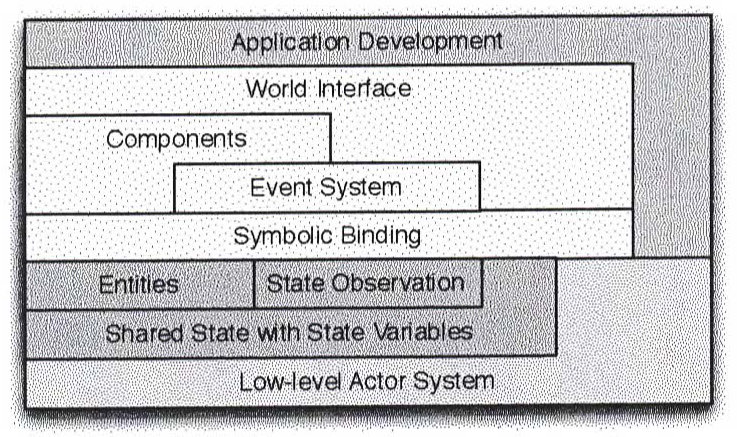
\includegraphics[width=90mm]{bilder/siris_arch.png}
\caption{Systemstruktur von SIRIS \autocite{SimulatorX}}
\label{fig:sirisarch}
\end{figure}

Die funktionalen Komponenten sind in SIRIS stark voneinander entkoppelt, da alle Kommunikation über eine einheitliche Schnittstelle, das \textit{World Interface}, läuft. Das World Interface hat hierbei vier Aufgaben (zitiert nach \autocite[48]{WorldInterface}):
\begin{enumerate}
    \item Benachrichtigung über Änderungsereignisse relevanter Simulationszustände
    \item Ausführen von Aktionen zur Änderung relevanter Simulationszustände
    \item Verarbeitung von Anfragen an relevante und beliebige Simulationszustände
    \item Konfiguration relevanter Ereignisse und möglicher Aktionen
\end{enumerate}
In SIRIS wird der "`Weltzustand"' in einzelne Zustandsvariablen zerlegt, die einzelnen Entitäten (beispielsweise 3D-Modelle) zugeordnet werden können und man somit ein objektzentriertes Weltmodell erhält \autocite[50]{WorldInterface}. Sowohl Entitäten als auch Actors haben lediglich Referenzen auf die Zustandsvariablen, siehe Abbildung \ref{fig:sirisactors}.
\begin{figure}
\centering
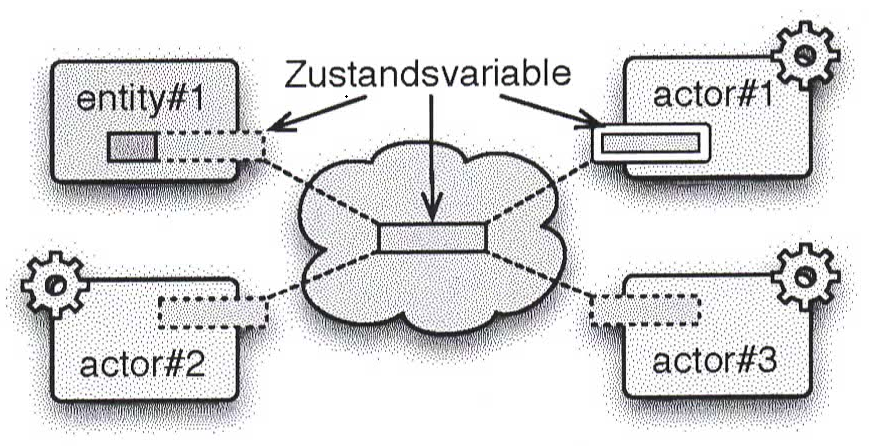
\includegraphics[width=80mm]{bilder/siris_actors.png}
\caption{Referenzierung in SIRIS \autocite{WorldInterface}}
\label{fig:sirisactors}
\end{figure}

Die Architektur von SIRIS basiert auf dem \textit{Actor Pattern}. Actors sind im Gegensatz zu Threads eine high-level Abstraktion von isoliert laufenden, nebenläufigen Prozessen. Jeder Actor kann über Nachrichten mit anderen, ihm bekannten Actors kommunizieren, hat aber keinerlei Einfluss darauf wie, wann und ob die angesprochenen Actors auf die Nachrichten reagieren. Actors sind sehr sicher, da sie keinen gemeinsamen Status haben. Dies vereinfacht den Umgang mit nebenläufigen Prozessen deutlich (für eine sehr gute Einführung siehe \autocite{ActorsInScala}).

In SIRIS gibt es auch ein Event Handling-Modell über das Actors, die sich für Änderungen an einer Zustandsvariable interessieren, benachrichtigt werden sobald sich diese verändert.
\lstset{language=Scala}
\begin{lstlisting}[caption={Registrieren einer Callbackfunktion zur Änderungsüberwachung einer Zustandsvariablen}, label={lst:siriscallback}]
handleEntity('myEntity)(entity => entity match {
  case Some(e) => {
    e.get(Transformation) match {
      case Some(sVar) => observe(sVar, (matrix: Mat4x4) => {
        // Do something with the matrix
      })
      case None => {
        // The entity 'myEntity does not reference a status variable (sVar) of type Transformation.
      }
    }
  case None => {
    // Entity with the name 'myEntity was not found
  }
})
\end{lstlisting}
Listing \ref{lst:siriscallback} mag gerade für Scala-Unerfahrene auf den ersten Blick etwas überfordern. Im Kapitel \ref{chap:umsetzung} wird erläutert was sich genau dahinter verbirgt. Auf die Methode \texttt{handleEntity} wird etwas weiter unten noch kurz eingegangen.

SIRIS verfügt über eine eingebaute Knowledge Representation Layer (Wissensrepräsentationsebene). Entitäten und Zustandsvariablen werden auf Anwendungsebene mit Hilfe der Web Ontology Language (kurz OWL, siehe \autocite{OWL}) beschrieben. Dies deshalb, da die funktionalen Komponenten des Softwaresystems intern häufig eine andere Repräsentation, beispielsweise einer Entität, benötigen und in anderer Weise auf Attribute zugreifen müssen als andere Komponenten. Die Beschreibung liefert einen global gültigen Datentyp und die funktionalen Komponenten erhalten einen für sie konvertierten, lokalen Datentyp mit dem sie arbeiten können. Hierdurch können die Komponenten autonom arbeiten und sind nicht von den lokalen Datentypen in anderen Komponenten abhängig \autocite[44]{EnhancedDecoupling}. Entitäten können hierbei aus verschiedenen Aspekten bestehen, wie beispielsweise einem 3D-Mesh und einer Hüllgeometrie\footnote{Wird beispielsweise von der Physik benötigt, um festzustellen ob ein Objekt mit einem anderen kollidiert ist}. Für das Erstellen von Zustandsvariablen und Entitäten gibt es eine Methode namens \texttt{realize}. In Listing \ref{lst:sirisfassrealisierung} ist ein Beispiel für das Erstellen einer 3D Geometrie-Entität (konkret ein Fass) beschrieben. Der dort dargestellte Code gehört zum Barrelstack-Benchmark von SIRIS und wurde für bessere Lesbarkeit etwas angepasst. So werden \texttt{scale} und \texttt{transform} in Wirklichkeit natürlich mit konkreten Werten initialisiert.
\lstset{language=Scala}
\begin{lstlisting}[caption={Erstellen einer Entität über eine Entitätsbeschreibung}, label={lst:sirisfassrealisierung}]
realize(
  EntityDescription(
    ShapeFromFile(
      file = "assets/vis/barrel/barrel3.dae",
      scale = ConstMat4(...),
      transformation = ReadFromElseWhere
    ),
    PhysCylinder(
      transform = ConstMat4(...),
      radius = 3.0,
      height = 5.0,
      align = Axis.Z,
      mass = 10.0
    )
  ),
  (e : Entity) => println( "Created barrel")
)
\end{lstlisting}
Die \texttt{EntityDescription} enthält zwei Aspekte: ein 3D-Mesh, welches aus einer COLLADA-Datei gelesen wird \texttt{barrel3.dae}, und eine Hüllgeometrie \texttt{PhysCylinder}. Zudem wird eine Callback-Funktion bereitgestellt die aufgerufen wird, sobald die Entität erstellt wurde. In obigem Fall wird dann lediglich "`Created barrel"' auf der Konsole ausgegeben.

Die Registrierung von Entitäten, neuen Actors und Zustandsvariablen geschieht ebenfalls über einen Actor. Sie werden über Symbole, ein Konstrukt aus der Sprache Scala, registriert. Hierbei kann eine Komponente auch über mehrere Symbole registriert werden. Intern werden jedoch Universally Unique Identifiers (kurz UUIDs) verwendet. Diese ermöglichen die eindeutige Identifikation einer registrierten Komponente \autocite[51]{WorldInterface}.

Für jede registrierbare Komponente, sei es eine Zustandsvariable, ein Actor oder eine Entität, gibt es im World Interface eigene Methoden. Listing \ref{lst:sirisentityhandling} zeigt beispielsweise die Methoden für den Umgang mit Entitäten.
\lstset{language=Scala}
\begin{lstlisting}[caption={Methoden zum Registrieren, handlen und deregistrieren von Entitäten}, label={lst:sirisentityhandling}]
registerEntity(name: Symbol, e: Entity) {
  // Register an entity with the given name
}

unregisterEntity(e: Entity) {
  // Unregister a given entity
}

handleEntity(name: Symbol)(handler: Option[Entity] => Any ) {
  // Handle an entity (if exists) with the given name and the given handler function (callback function)
}
\end{lstlisting}
Durch diese Konzentration auf den Zustand von Objekten werden zwei für die Softwarequalität wichtige Aspekte erreicht \autocite[305]{GuruMeditation}:
\begin{itemize}
    \item \textbf{Starke Kohäsion}\\
Kohäsion beschreibt wie gut die in einem Softwaresystem enthaltenen funktionalen Komponenten ihre jeweiligen Aufgaben abbilden. Starke Kohäsion meint hierbei dass jede Komponente nur die von ihr zu leistende Aufgabe erledigt. Ähnlich ist das Unix-Prinzip, ausgedrückt von Doug McIlroy, einem der Begründer der Unix-Philosophie: \begin{quote}"`This is the Unix philosophy: Write programs that do one thing and do it well.[\ldots]"'\footnote{zitiert nach \url{http://www.faqs.org/docs/artu/ch01s06.html} (besucht am 19. August 2012)}\end{quote}
    \item \textbf{Niedrige Kopplung}\\Kopplung beschreibt wie stark funktionale Komponenten in einem Softwaresystem voneinander abhängen. Niedrige Kopplung meint hierbei dass einzelne Komponenten ihre Aufgaben völlig autark und isoliert erledigen können und bestenfalls nichts von der Existenz anderer Komponenten wissen (müssen).
\end{itemize}
SIRIS bildet daher eine moderne, sehr gut erweiterbare Plattform in der sich Komponenten leicht austauschen oder entfernen lassen, ohne dabei andere Komponenten oder gar das zugrunde liegende System verändern zu müssen. Dies erhöht die Wartbarkeit und verringert sowohl die Komplexität selbst geschriebener Anwendungen und verbessert die Lernkurve für neue Entwickler die später in ein Projekt einsteigen und das System (oder zumindest den Teil des Systems an dem sie mitarbeiten werden) erst kennenlernen müssen.